\subsection{Documentação Typedoc}
Para a documentação de código foi utilizado \textit{typedoc}. Durante a implementação do \textit{typedoc} foi detetado que a categorização da documentação não estava funcional devido a um problema encontrado pelos programadores da ferramenta. Deste modo reduziu-se a versão para uma com a funcionalidade ativa, mas esta, não é compatível com a versão mais atualizada de \textit{Typescript}, pelo que, não foi possível explorar esta funcionalidade. Para contornar o problema foi explorada outra funcionalidade menos utilizada, esta permite converter qualquer documentação em módulos, estes podem ser categorizados, o problema é que é criado um modelo genérico do código, o qual não permite a fácil identificação das tipagens de \textit{scripts}. Estes módulos permitem também a categorizar, o que leva a um maior nível de organização da documentação.
Encontra-se no documento de anexos, no anexo 23 e 24, uma versão em maiores dimensões das Figuras~\ref*{type_doc} e \ref*{type_doc_det}.

\begin{figure}[htb]
 \centering
 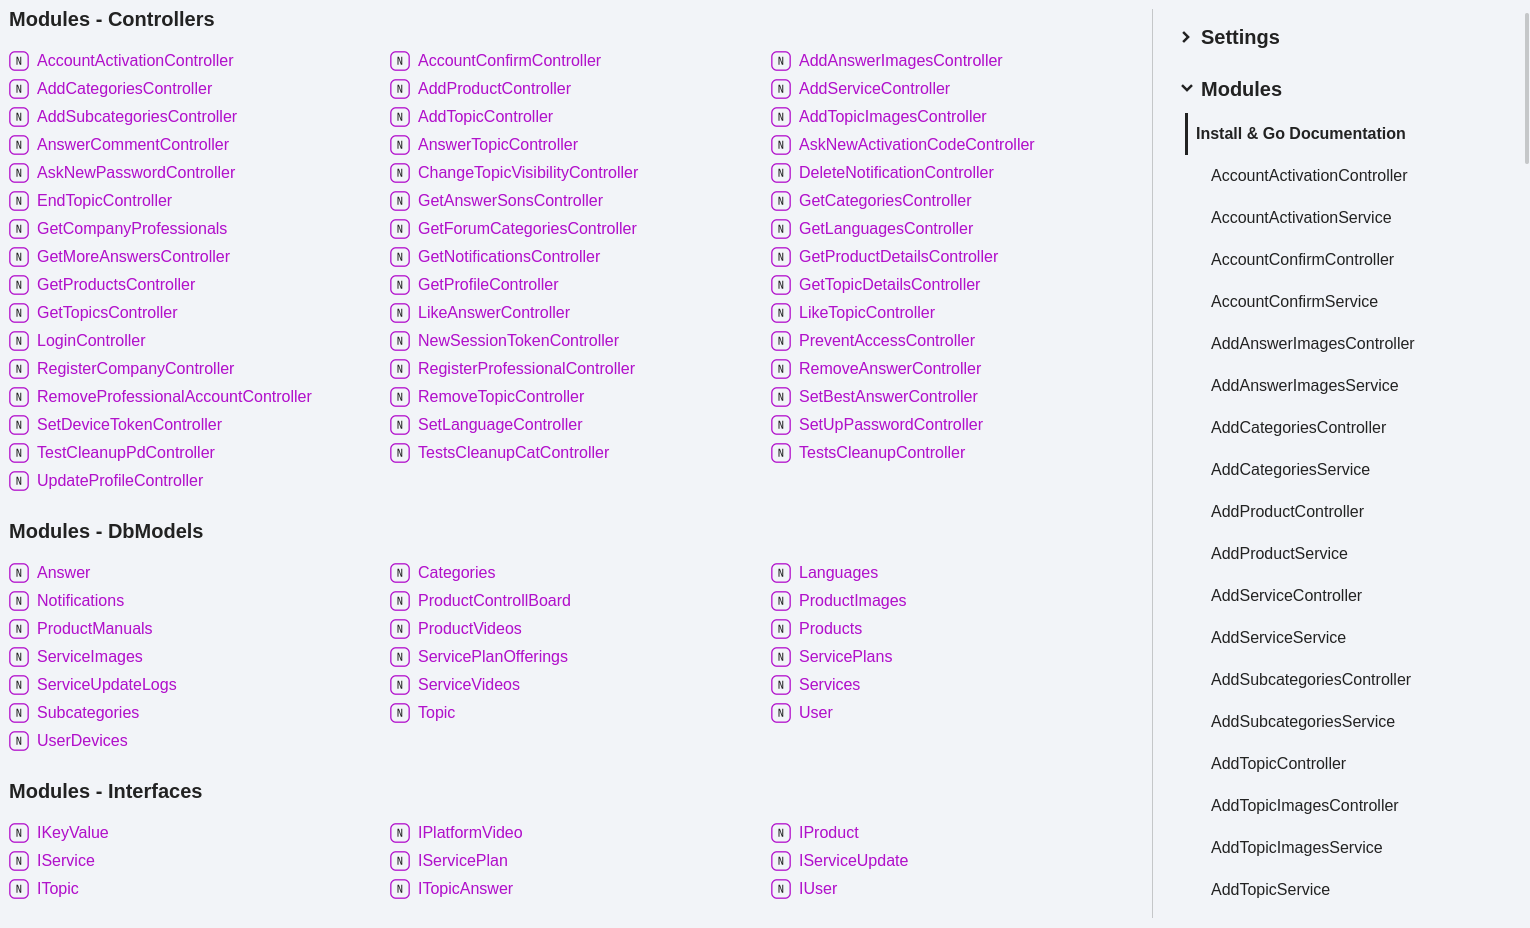
\includegraphics[width=0.75\textwidth]{images/implementacao/api/docs.png}
 \caption{Documentação \textit{typedoc}}
 \label{type_doc}
\end{figure}

\begin{figure}[htb]
 \centering
 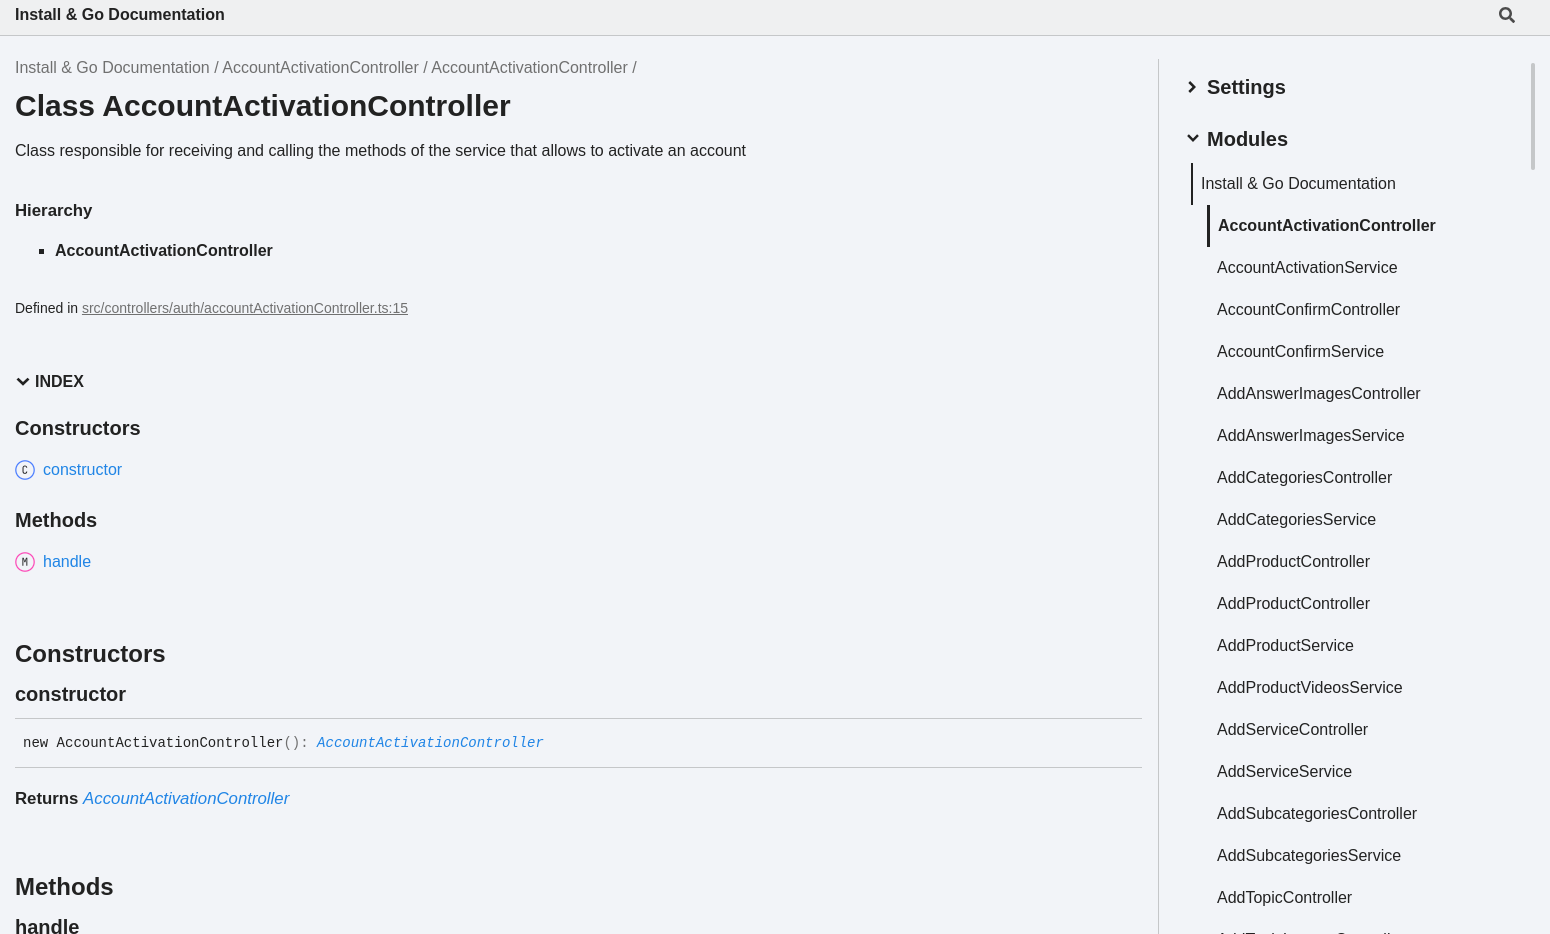
\includegraphics[width=0.75\textwidth]{images/implementacao/api/docs_det.png}
 \caption{Documentação de classe \textit{typedoc}}
 \label{type_doc_det}
\end{figure}

\newpage

\subsection{Documentação Swagger}
Apesar do \textit{swagger} disponibilizar a funcionalidade de gerar automáticamente documentação a partir de comentários de código, foram encontrados alguns problemas com esta funcionalidade, o que levou a que não fosse possível gerar a documentação. Portanto, optou-se por manter a documentação manualmente com o ficheiro \textit{\acrshort{json}}. Esta ferramenta oferece diversas funcionalidades como autenticação, definição de estruturas de dados para os serviços e exemplos de respostas. Estas funcionalidades foram exploradas o que gerou um bom suporte de documentação para qualquer utilizador.
Encontra-se no documento de anexos, no anexo 25 e 26, uma versão em maiores dimensões das Figuras~\ref*{fig:67} e \ref*{fig:68}.
\begin{figure}[htb]
 \centering
 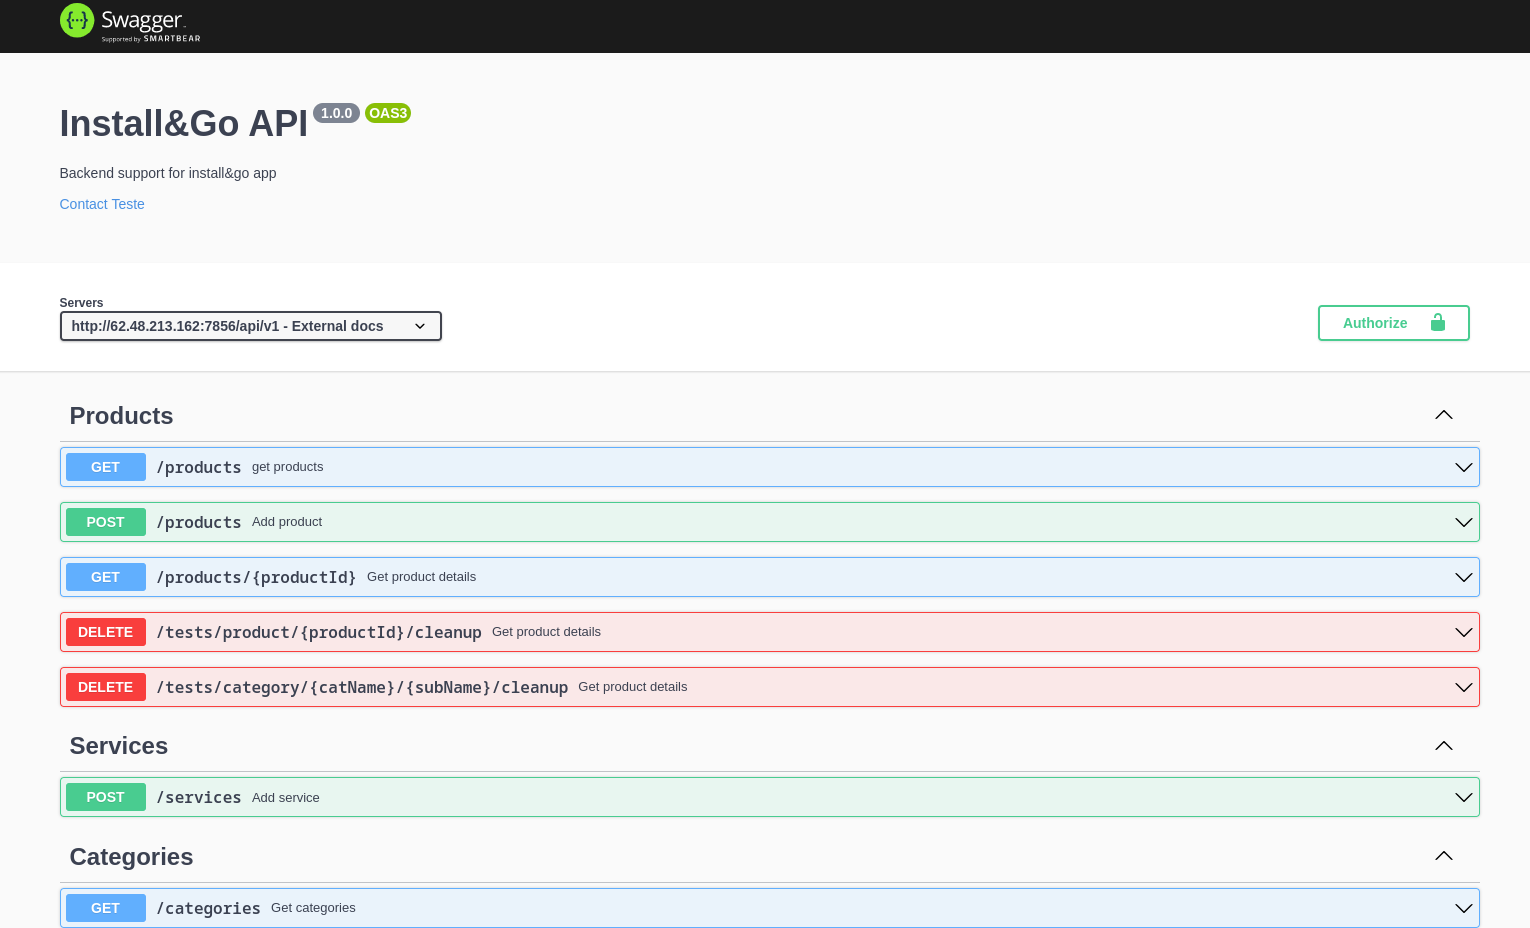
\includegraphics[width=0.7\textwidth]{images/implementacao/api/swagger_intro.png}
 \caption{Documentação swagger}
 \label{fig:67}
\end{figure}

\begin{figure}[htb]
 \centering
 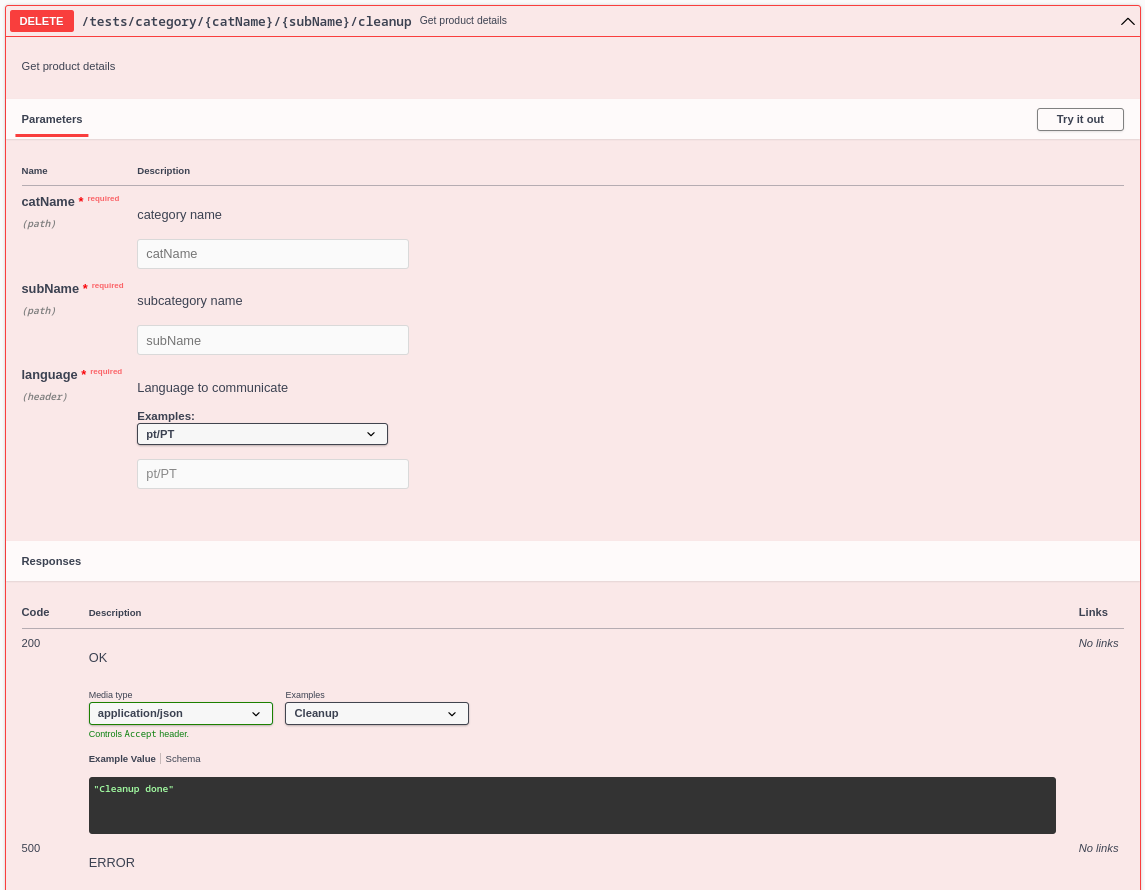
\includegraphics[width=0.5\textwidth]{images/implementacao/api/swagger_pedido.png}
 \caption{Exemplo de documentação de serviço}
 \label{fig:68}
\end{figure}